\section{Task 2}
\begin{document}
Die folgende Abbildung zeigt die durchschnittliche Laufzeit des Minimax Algorithmus und des AlphaBeta Algorithmus mit und ohne Movesorting auf 10 verschiedenen Maps:

\begin{figure}[h]
	\begin{center}
		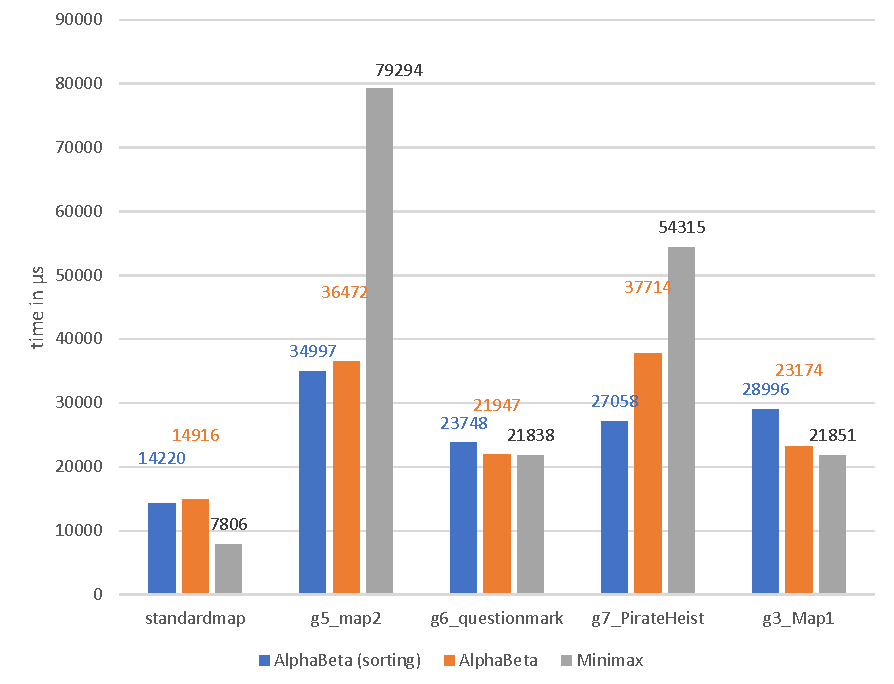
\includegraphics{Depth_1_avgtime.pdf}
		\caption{Durchschnittszeit bei Tiefe 1}
		\label{fig::avgtime Depth1}
	\end{center}
\end{figure}
\begin{figure}[h]
	\begin{center}
		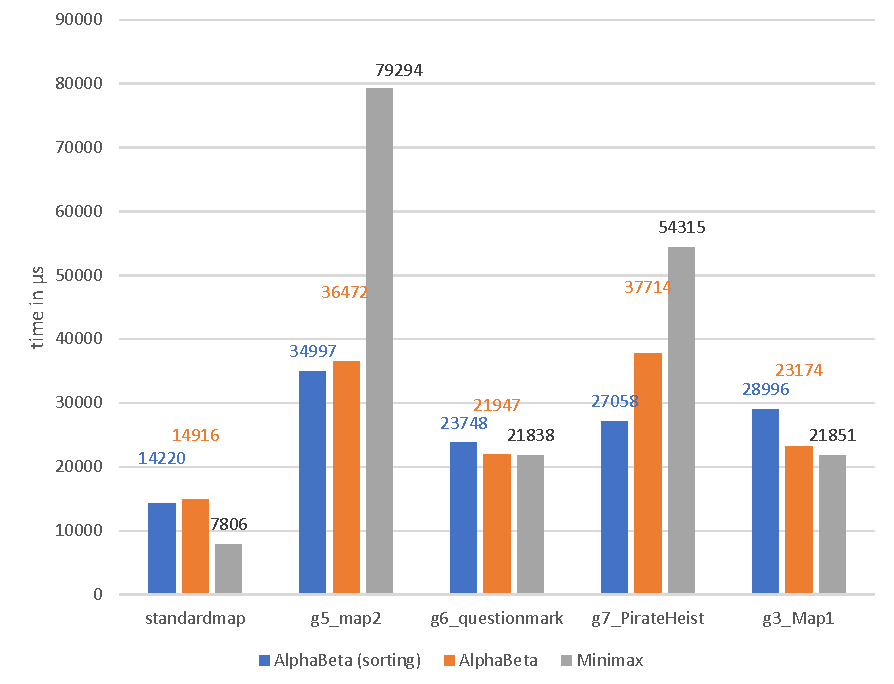
\includegraphics{Depth_2_1_avgtime.pdf}
		\caption{Durchschnittszeit bei Tiefe 2 (1/2)}
		\label{fig::avgtime Depth2.1}
	\end{center}
\end{figure}
\begin{figure}[h]
	\begin{center}
		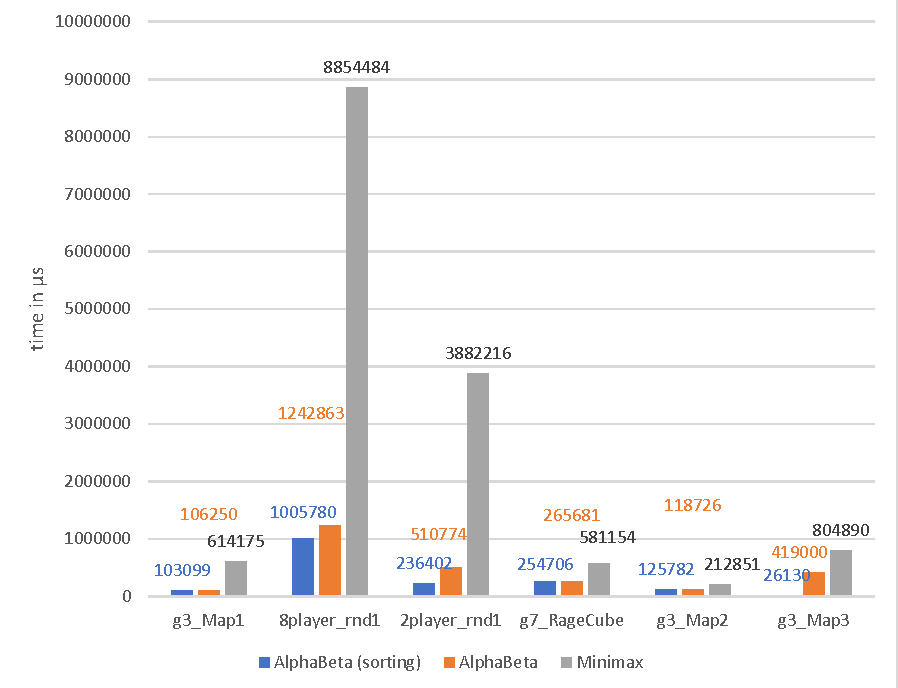
\includegraphics{Depth_2_2_avgtime.pdf}
		\caption{Durchschnittszeit bei Tiefe 2 (2/2)}
		\label{fig::avgtime Depth 2.2}
	\end{center}
\end{figure}
Aus figure 1, 2 und 3 ist erkennbar, dass vorallem bei Tiefe 2 der AlphaBeta Algorithmus mit Movesorting schneller arbeitet als der Minimax Algorithmus.
Jedoch gibt es auch des öfteren Fälle, wo der Minimax schneller als der AlphaBeta Algorithmus ist.

\begin{figure}[h]
	\begin{center}
		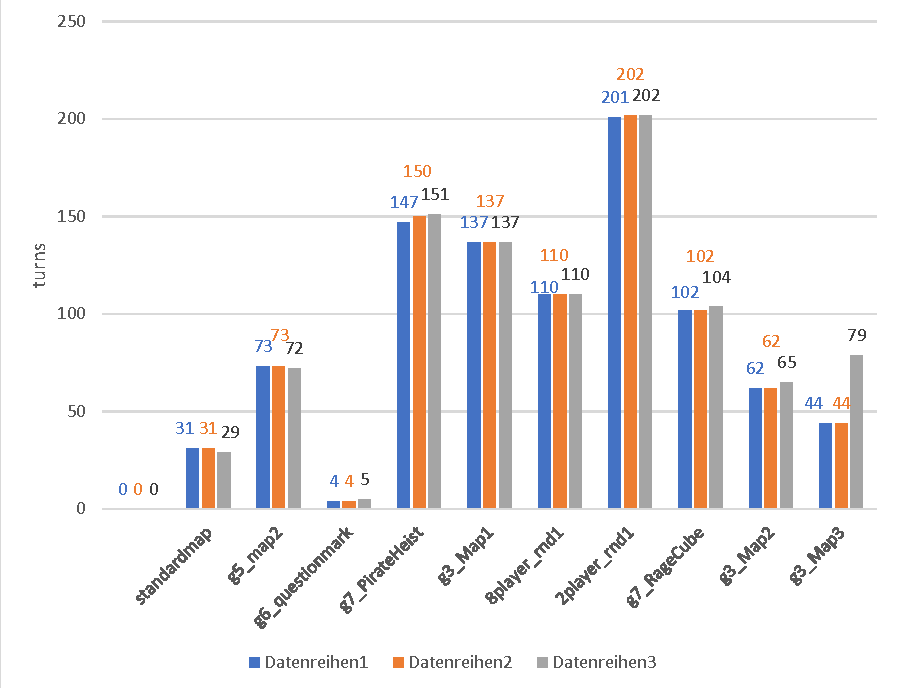
\includegraphics{Depth_1_turns.pdf}
		\caption{Anzahl der Züge bei Tiefe 1}
		\label{fig::turns Depth1}
	\end{center}
\end{figure}

Aus der Grafik 4 wird ersichtlich, dass die verschiedenen Algorithmen unterschiedlich viele Züge auf der gleichen Map registrieren bis das Spiel endet. Daher lässt es sich feststellen, dass nicht die gleichen Spiele gespielt werden und somit auch die Anzahl der besuchten Knoten sich unterscheiden. 



\end{document}
